%************************************************
\chapter{Reflectively Learning to Control}
\label{chapter:reflectively_learning_to_control}
%************************************************

In order to demonstrate my solution to the problem of reflectively
learning-to-control, my examples will be within the physical block
building domain shown in \autoref{figure:an_example_problem_domain}.

\begin{figure}
\begin{center}
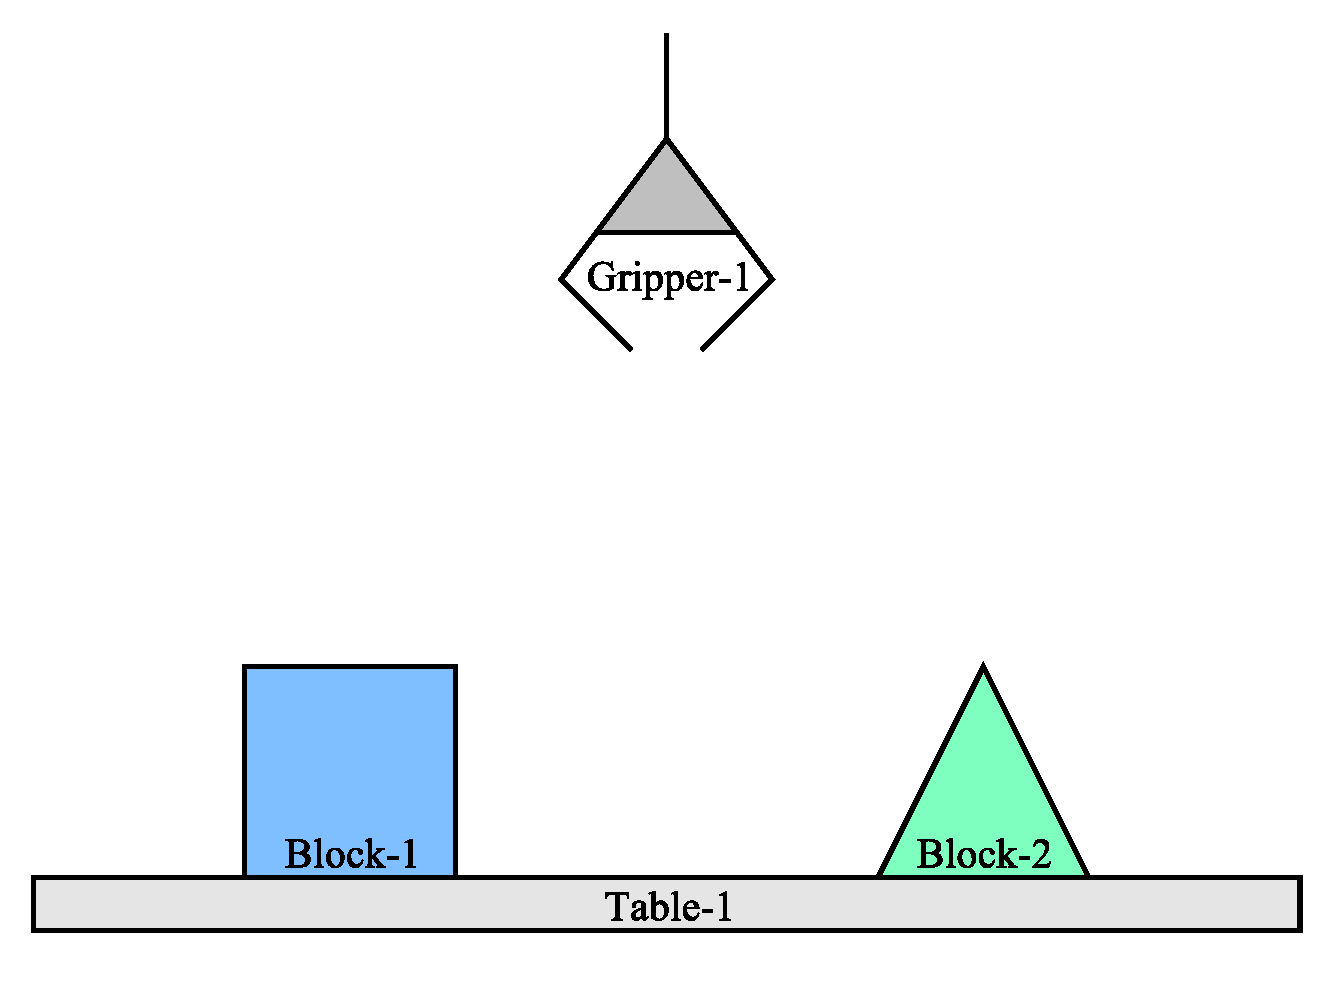
\includegraphics[width=8cm]{gfx/blocks_world_example-1}
\end{center}
\caption[An example problem domain.]{An example problem domain.}
\label{figure:an_example_problem_domain}
\end{figure}

\section{The Physical Knowledge-Base}

The block building domain is a simulation based on two-dimensional
ridid-body physical laws, including floating point numerical
representations for object positions, velocities and accellerations.
These numerical representations and the processes that manipulate them
are part of the $\text{reflective}^0$ physical layer of the model, but
in order to focus the efficiency of the procedural reflection, a much
simpler relational graph representation has been specifically
represented in semantic frame-based objects in a semantic
knowledge-base, referred to as the \emph{physical knowledge-base}.
The physical knowledge-base includes objects with shapes, colors, and
multiple prepositional spatial relationships.
{\mbox{\autoref{figure:implemented_physical_knowledge}}} shows the
physical knowledge-base.
\begin{sidewaysfigure}
\begin{center}
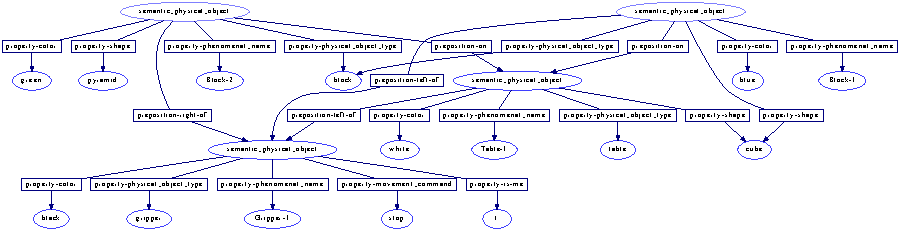
\includegraphics[width=24cm]{gfx/implemented_physical_knowledge}
\end{center}
\hspace{4cm}\parbox{15cm}{\caption[The physical knowledge-base.]{The
    physical
    knowledge-base.}\label{figure:implemented_physical_knowledge}}
\end{sidewaysfigure}

\section{An Example Storyboard}

{\mbox{\autoref{figure:implemented_example_learning_storyboard}}}
shows a storyboard of the implemented example of second-order
learning.
\begin{figure}
\begin{center}
\begin{tabular}{p{4cm}p{4cm}p{4cm}}
1. 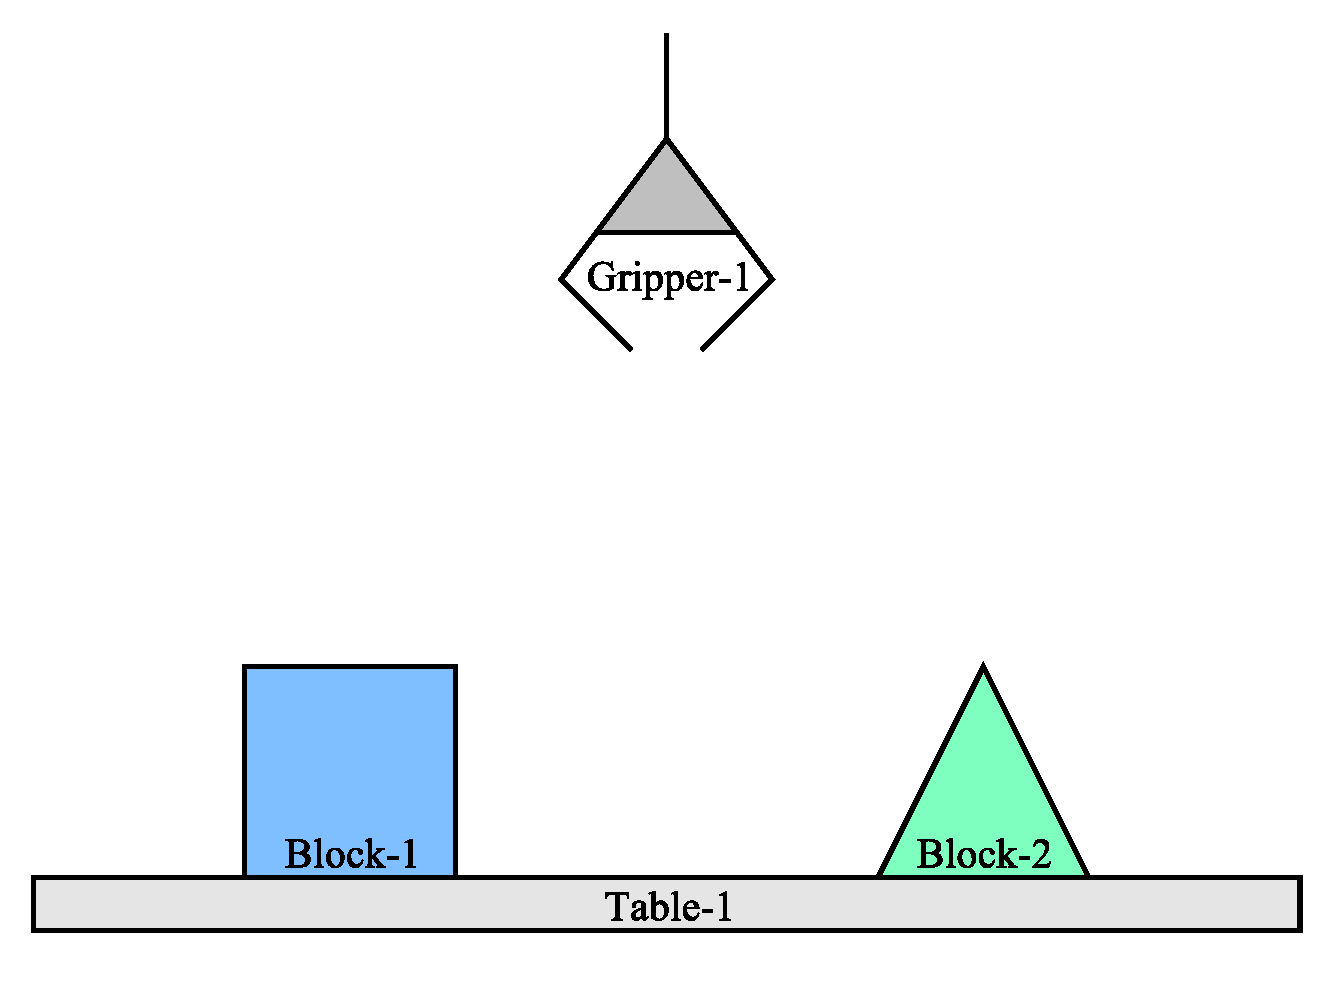
\includegraphics[width=4cm]{gfx/blocks_world_example-1}  & 2. 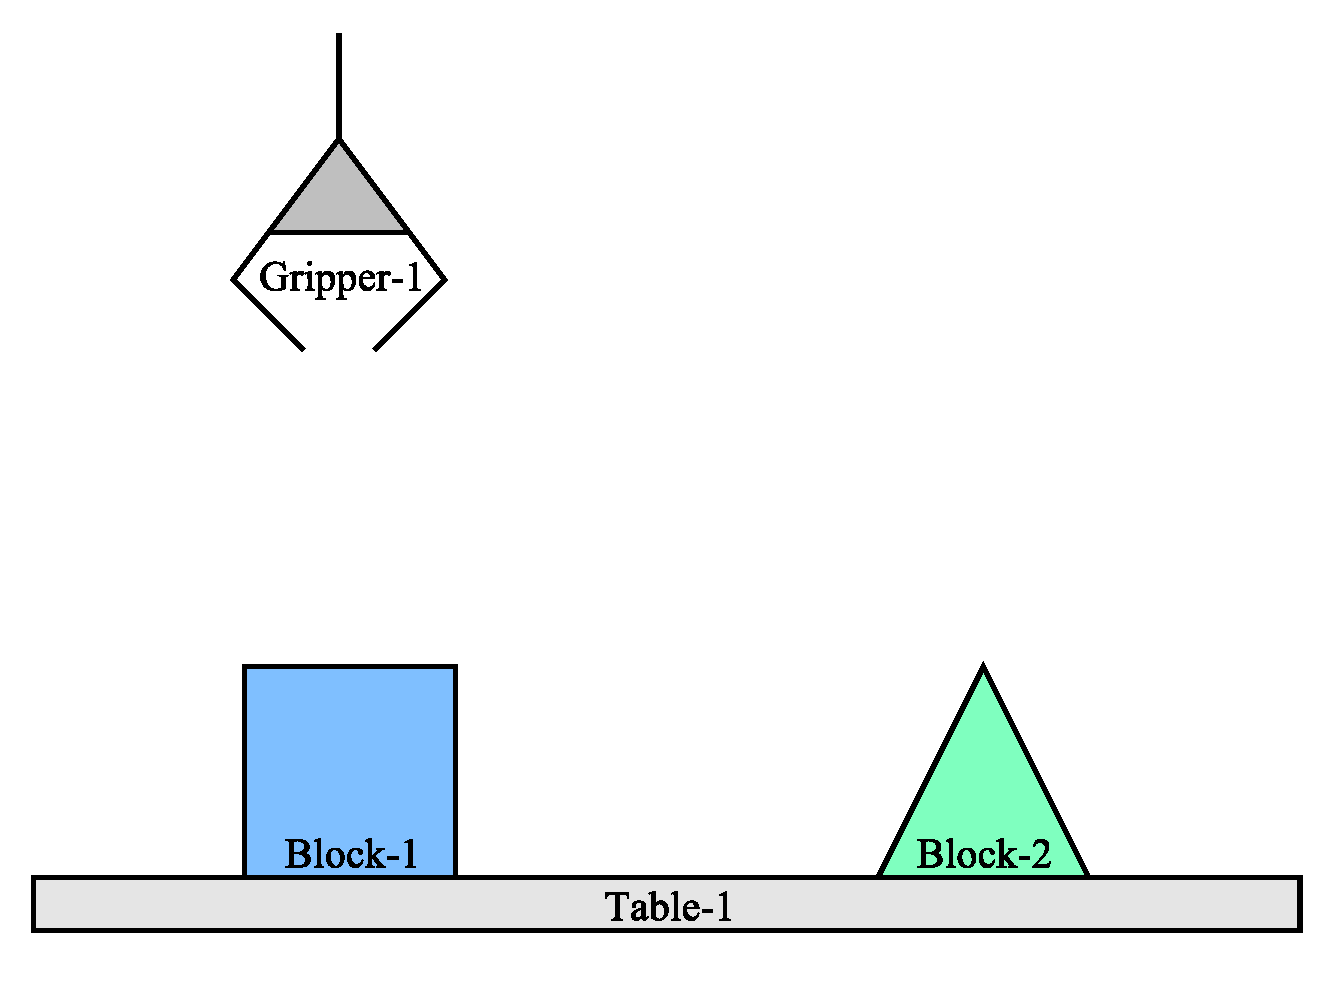
\includegraphics[width=4cm]{gfx/blocks_world_example-2}  & 3. 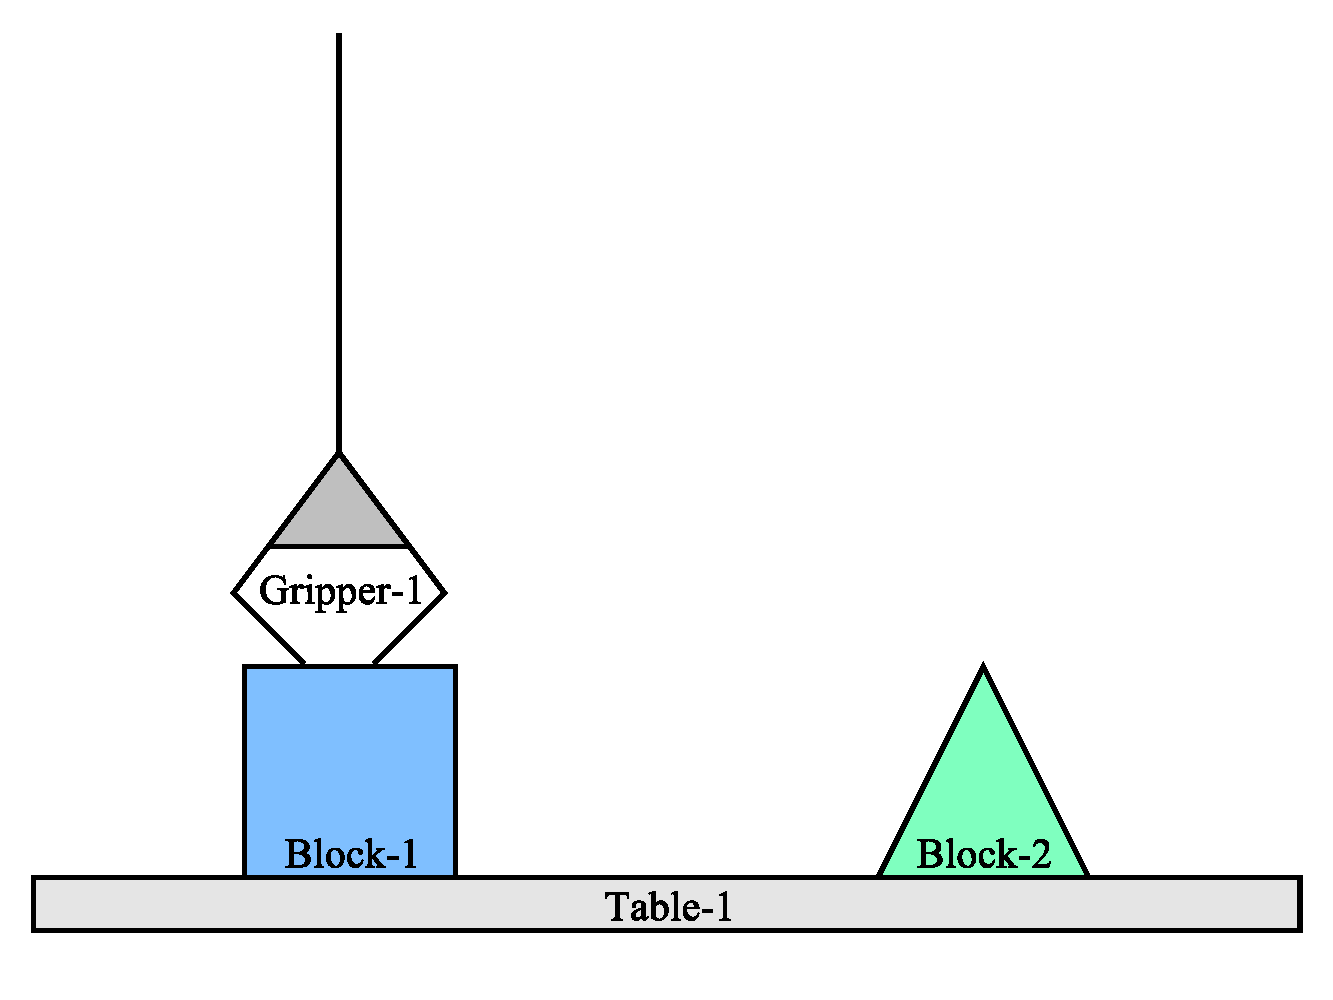
\includegraphics[width=4cm]{gfx/blocks_world_example-3} \\
4. 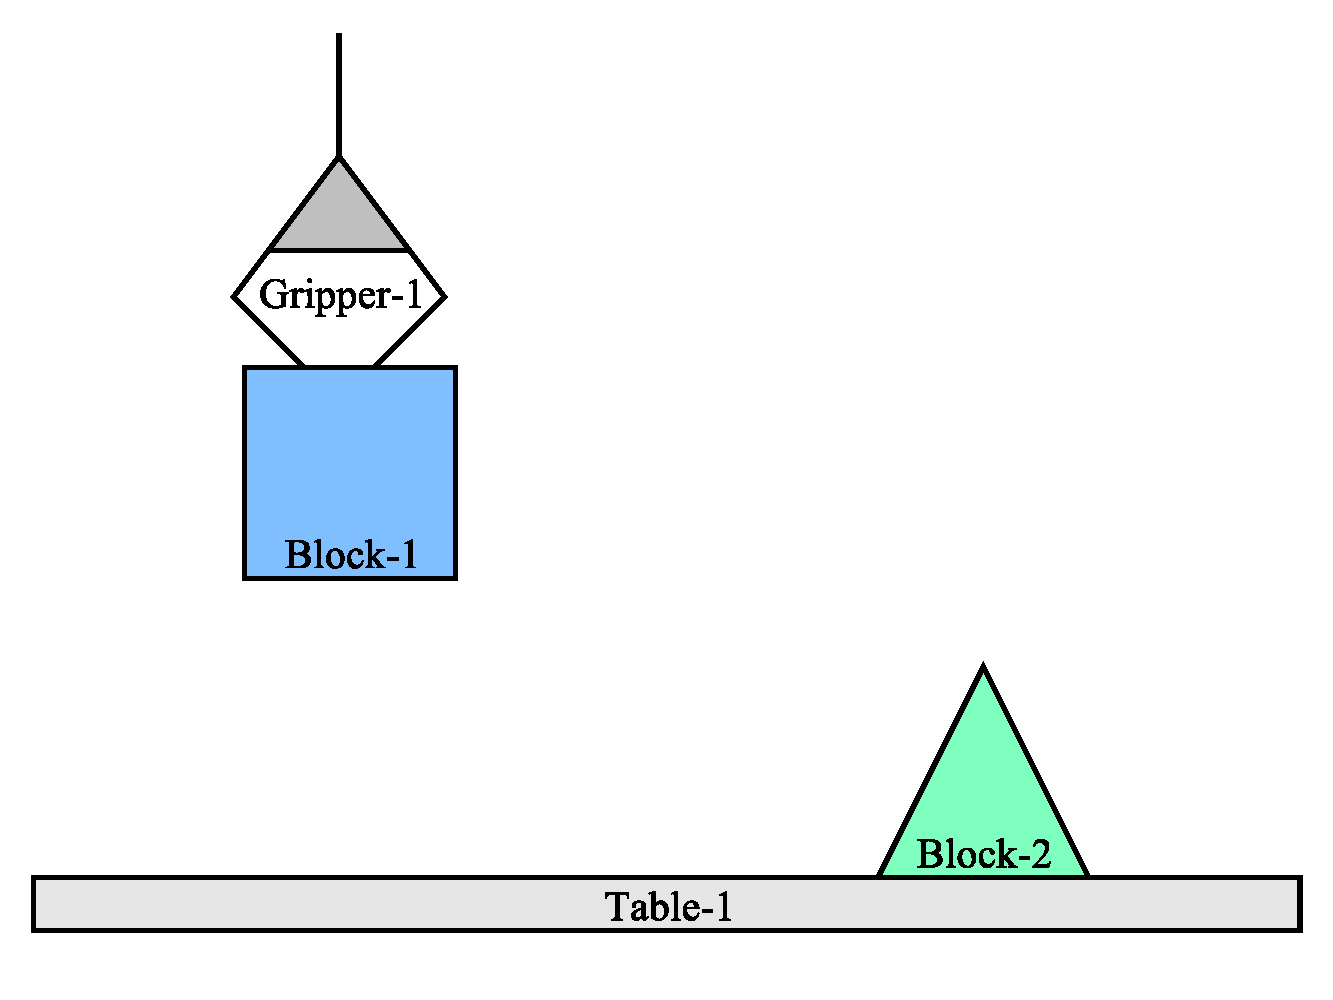
\includegraphics[width=4cm]{gfx/blocks_world_example-4}  & 5. 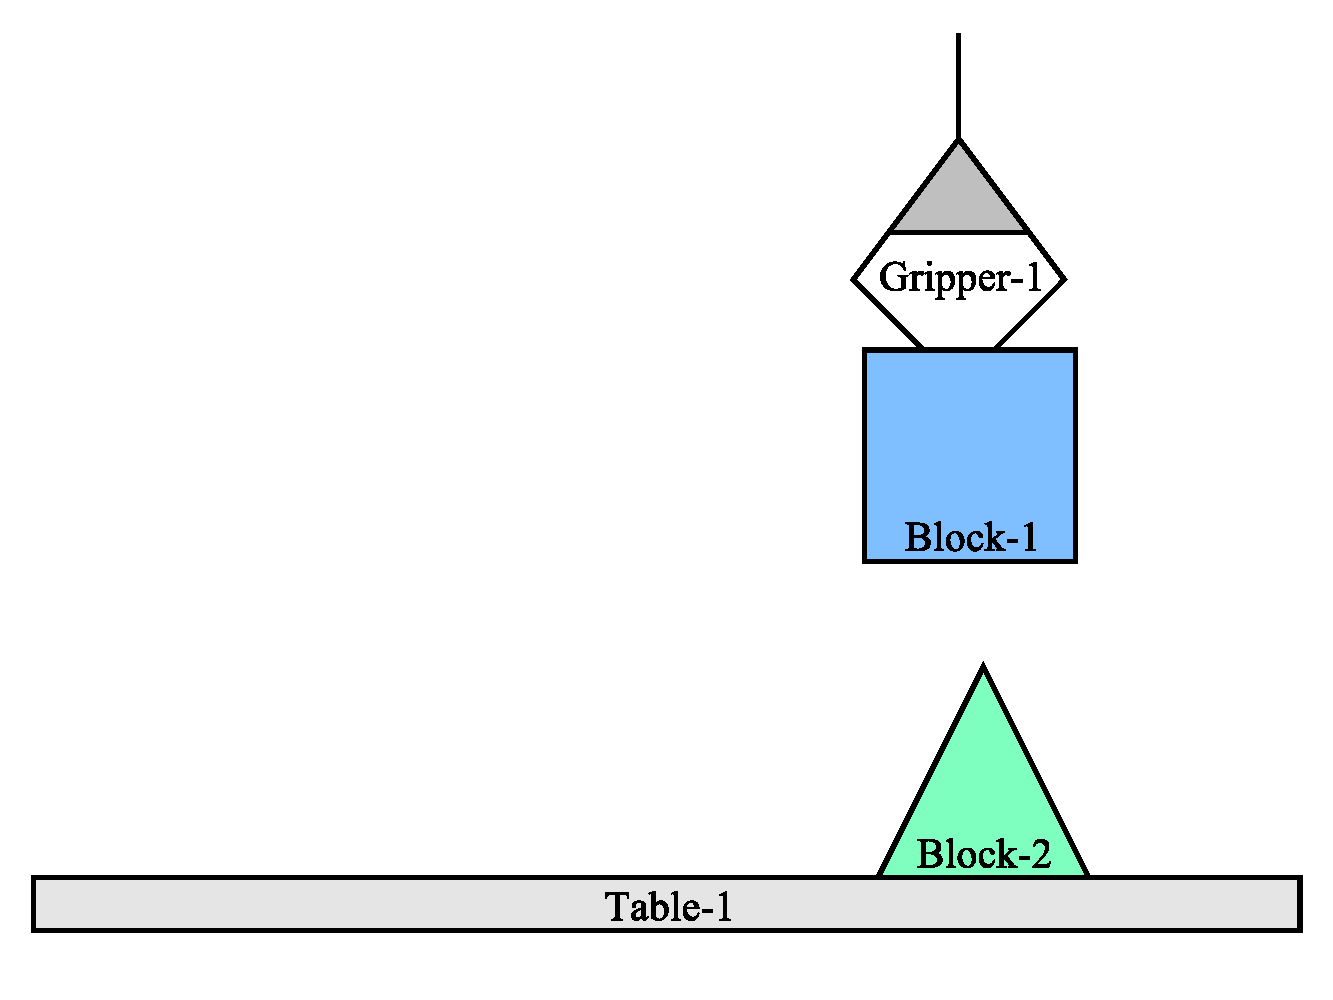
\includegraphics[width=4cm]{gfx/blocks_world_example-5}  & 6. 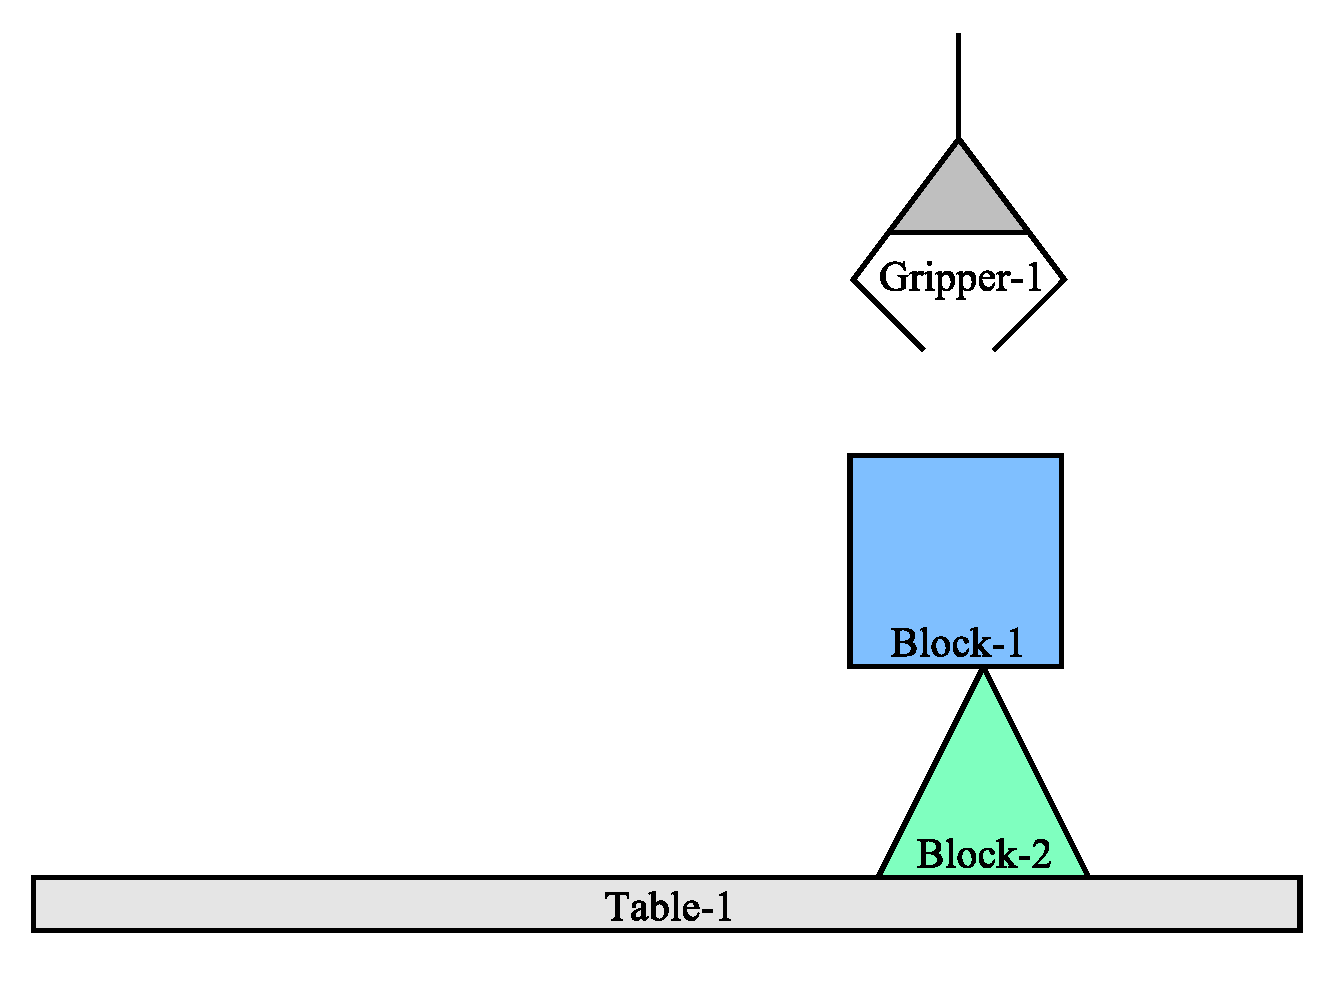
\includegraphics[width=4cm]{gfx/blocks_world_example-6} \\
7. 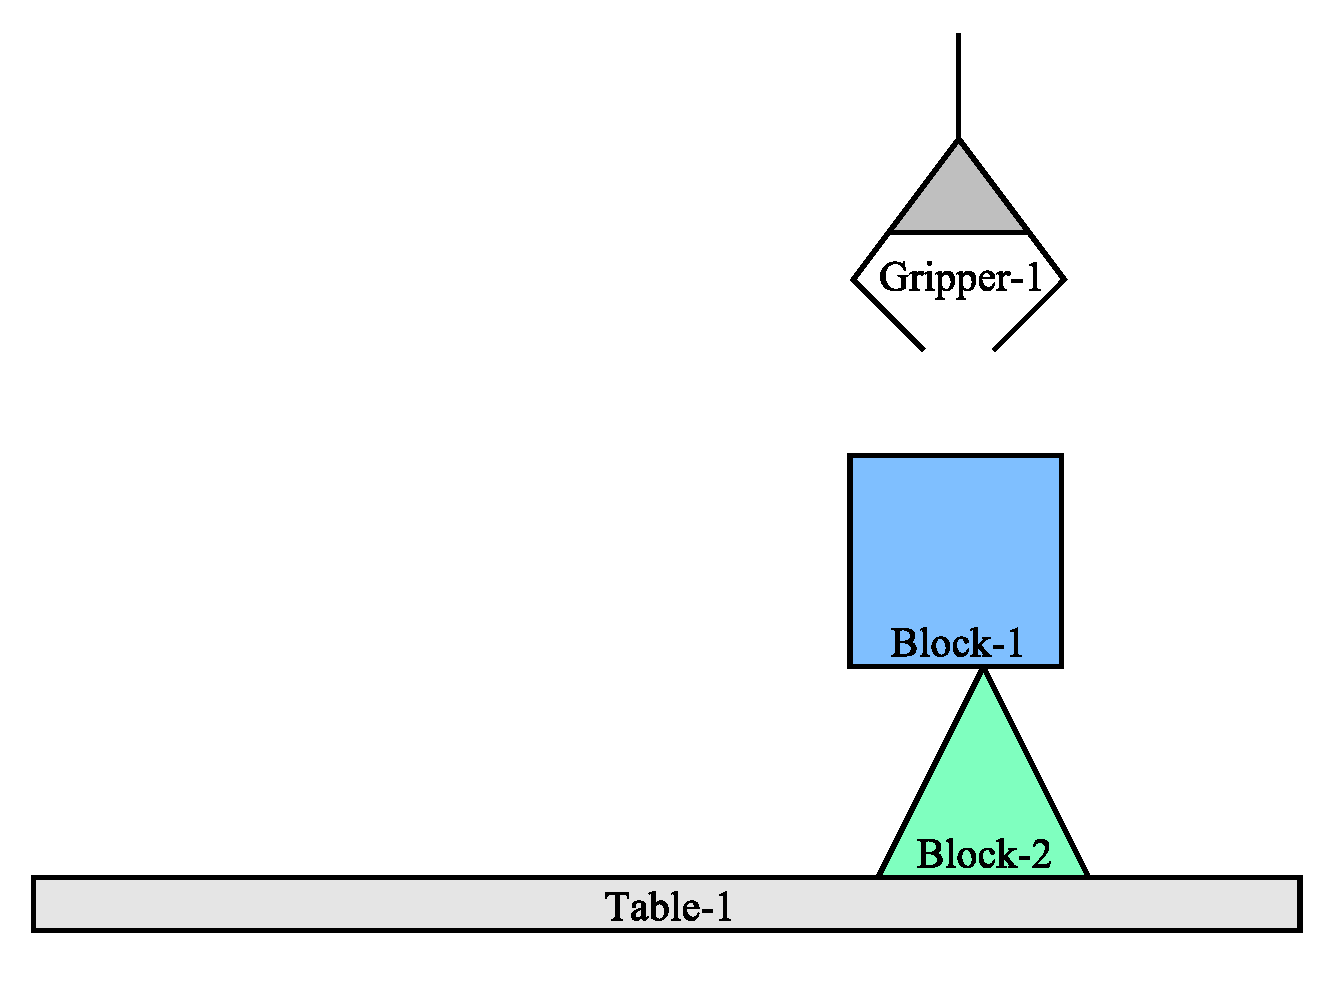
\includegraphics[width=4cm]{gfx/blocks_world_example-7}  & 8. 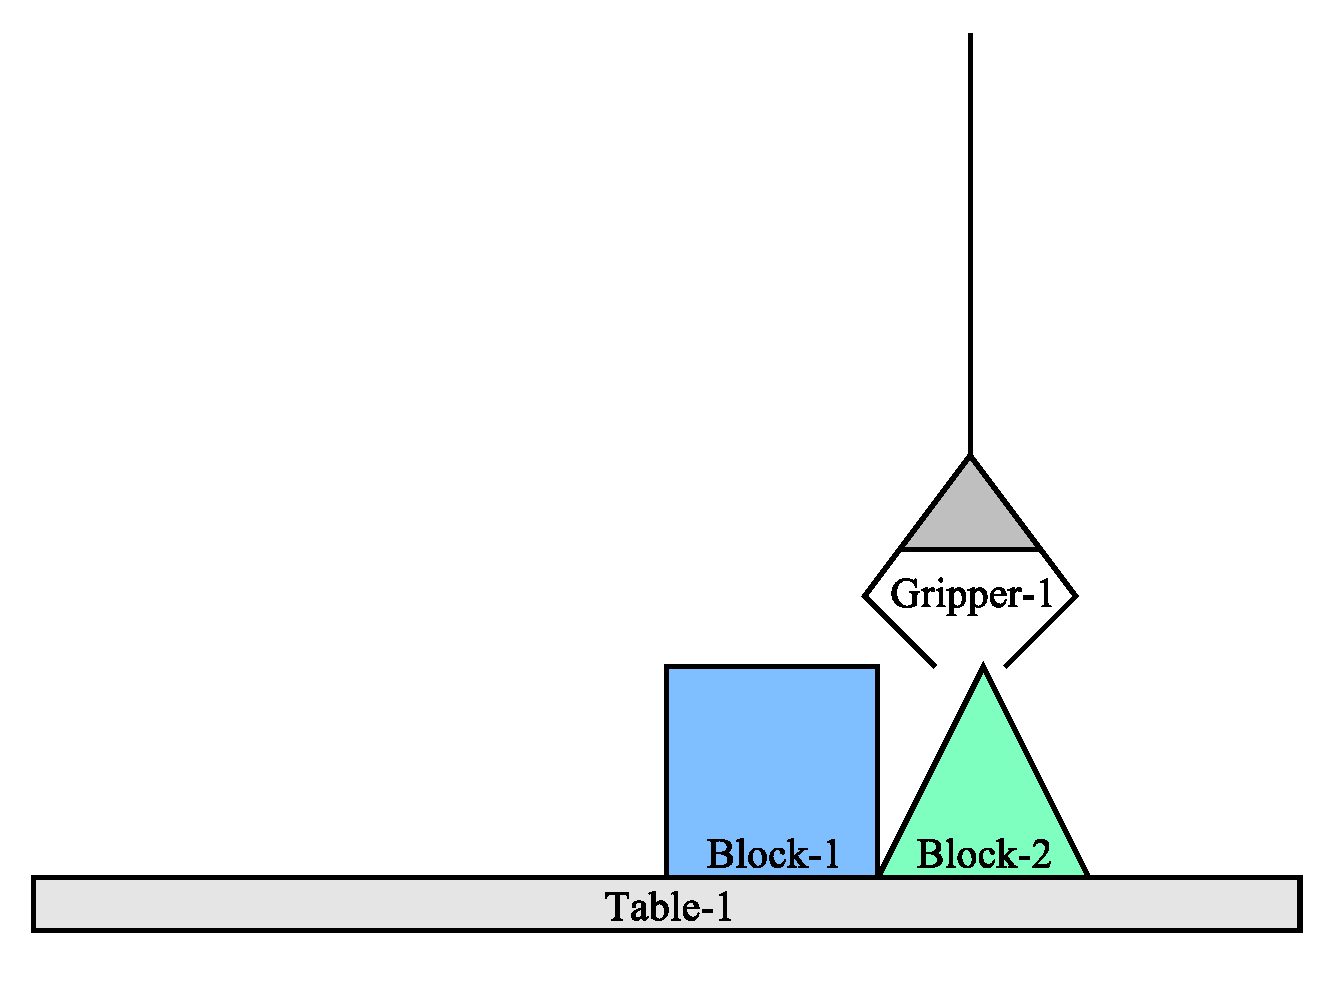
\includegraphics[width=4cm]{gfx/blocks_world_example-8}  & 9. 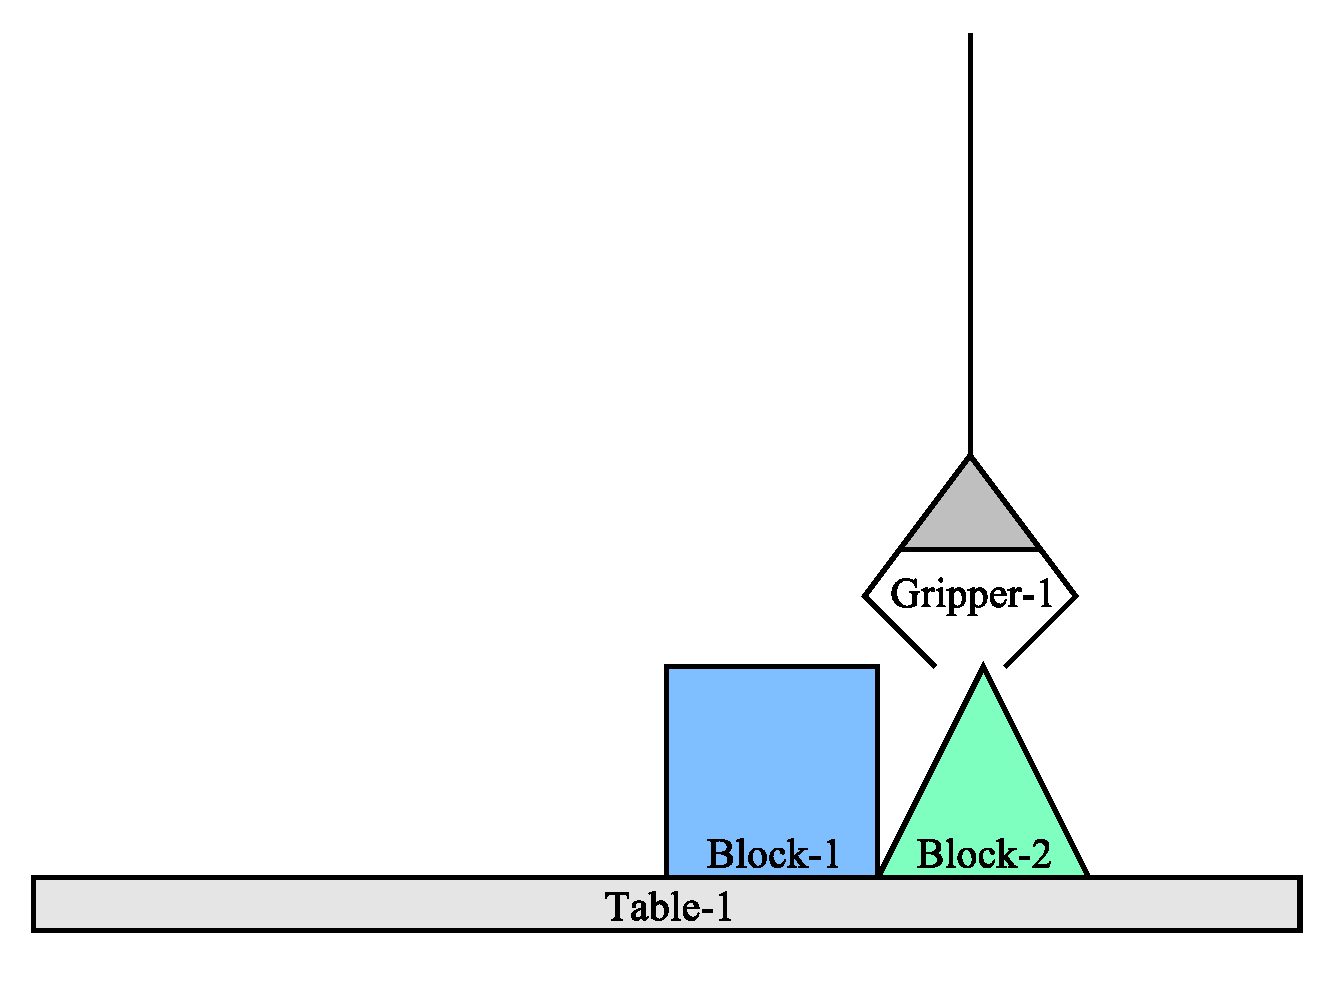
\includegraphics[width=4cm]{gfx/blocks_world_example-9} \\
10. 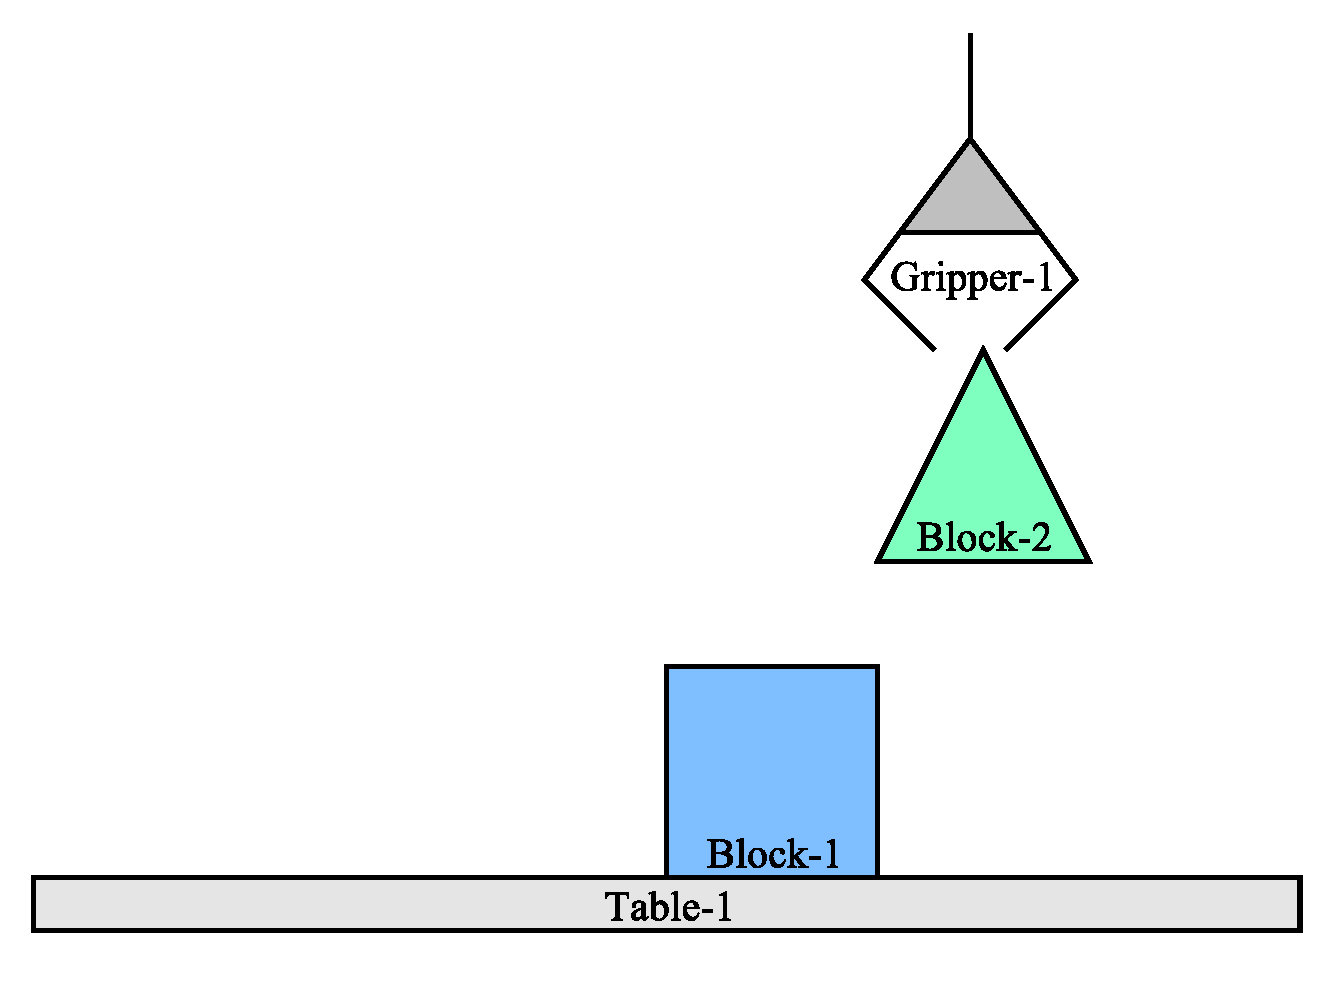
\includegraphics[width=4cm]{gfx/blocks_world_example-10} & 11. 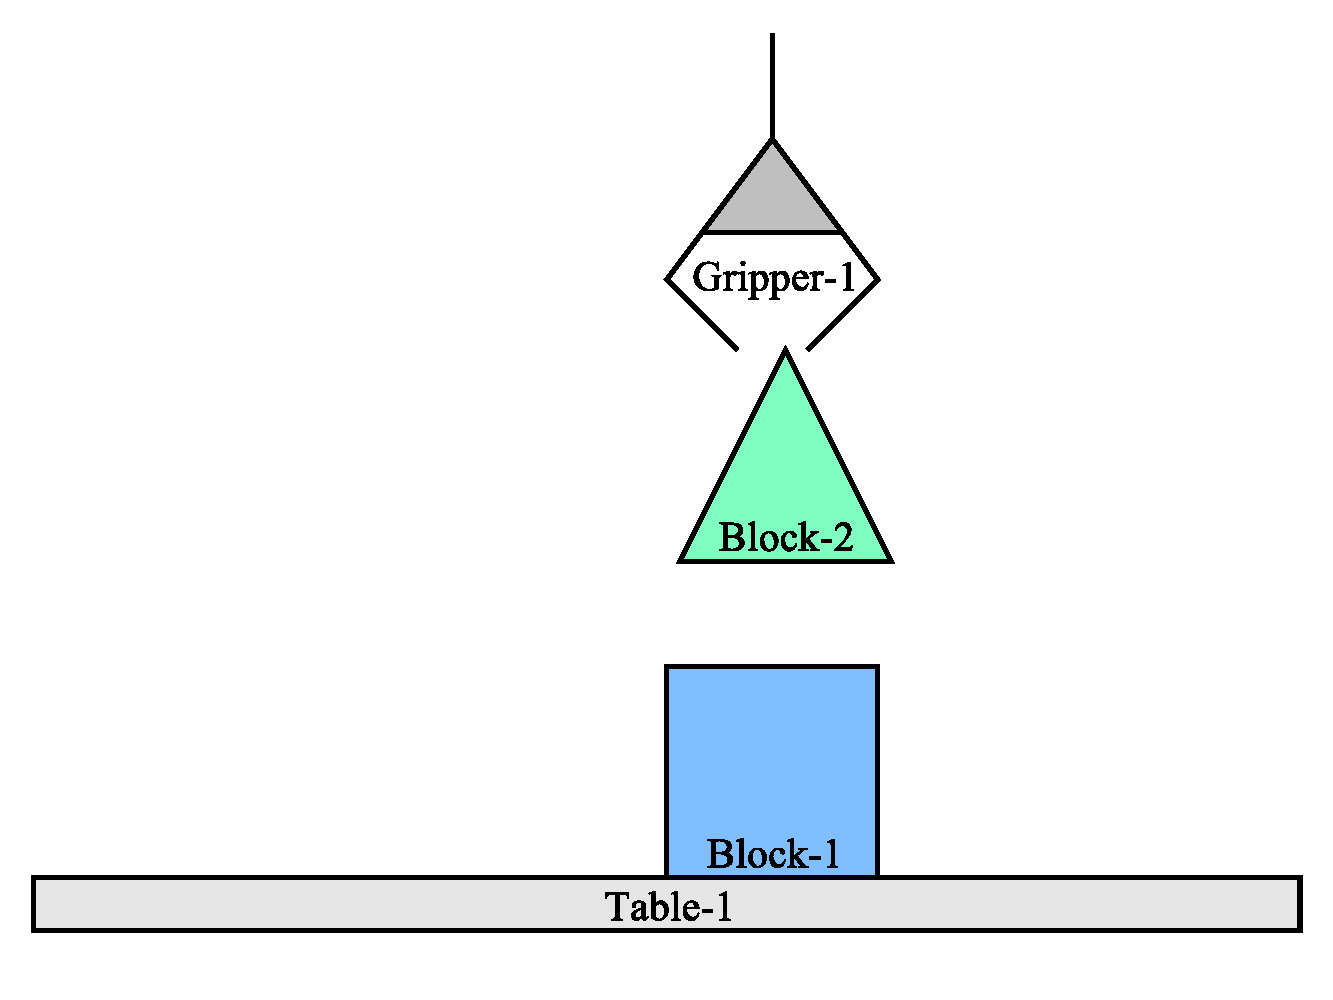
\includegraphics[width=4cm]{gfx/blocks_world_example-11} & 12. 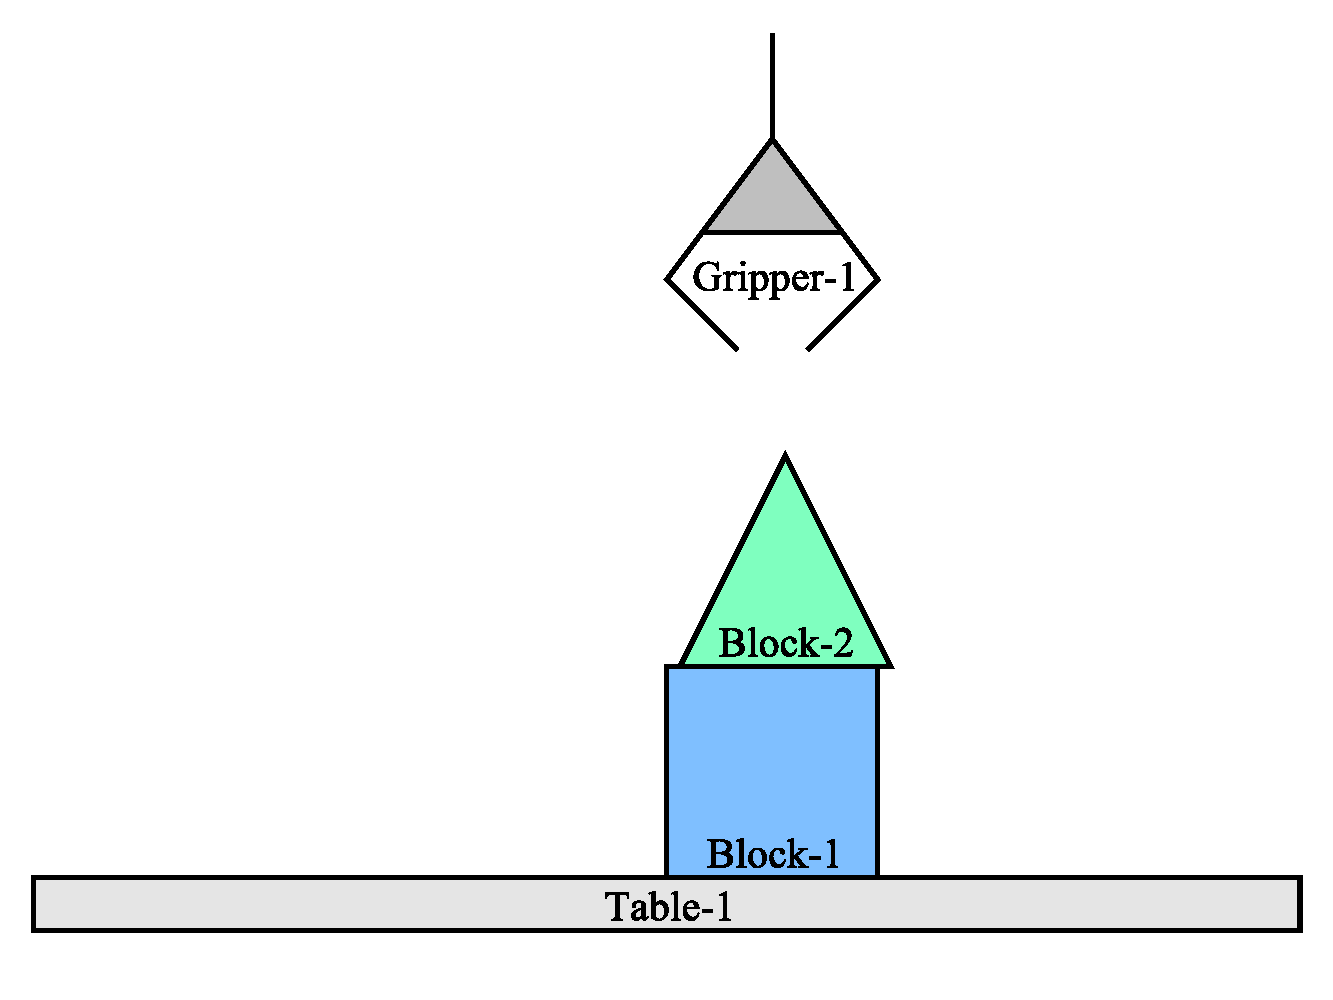
\includegraphics[width=4cm]{gfx/blocks_world_example-12}
\end{tabular}
\end{center}
\caption[A storyboard of the implemented example of second-order
  learning.]{A storyboarded example of second-order learning, where
  the goal is to create a stack of two blocks.  (1) A plan that is
  hypothesized to stack the square block on top of the triangular
  block is executed.  (2--8) The plan completes execution and results
  in the square falling off of the triangle, an expectation failure.
  (9) The second-order hypothetical heuristic is learned that predicts
  plan failure will result by executing plans that try to stack
  squares on top of triangles.  A plan that is hypothesized to stack
  the triangle on top of the square is executed.  (9-12) The second
  plan completes execution, accomplishing the physical goal.}
\label{figure:implemented_example_learning_storyboard}
\end{figure}

